% !TEX encoding = UTF-8
% !TEX TS-program = pdflatex
% !TEX root = ../tesi.tex
% !TEX spellcheck = it-IT

%**************************************************************
\chapter{Il modulo tema}
\label{cap:modulo-tema}
%**************************************************************

\intro{In questo capitolo verrà esposta l'implementazione e le fasi che hanno portato la creazione del modulo tema}
\section{scopo del modulo}
Il modulo tema è molto diverso come scopo e implementazione rispetto ai due precedentemente presentati: infatti questo modulo si basa sull'archetipo Share AMP e si come scopo non quello di aggiungere nuove funzionalità, ma quello di realizzare un tema gradevole e moderno, che vada ad aggiungersi a quello già presente nel KMS aziendale. La difficoltà maggiore di questo modulo è stata quindi quella di dover far convivere i due temi custom e implementare una soluzione che fosse facilmente manutenibile e permettesse anche il cambiamento del tema con la difficoltà minore possibile.
Era desiderabile, ma non è stato possibile, che ogni utente potesse scegliere un tema diverso.
\section{Realizzazione}
Nella implementazione dei due temi in una unica AMP è stato sfruttato il fatto, che nell'implementazione del tema precedente non era stato tenuto conto, che tutti i file di CSS del tema vengono automaticamente caricati assieme alla pagina share, quindi definendo lo stile con classi e ID (anche nuovi e non del tema) nei file principali del tema e non in file specifici per la pagina come nell'implementazione precedente, è possibile poter cambiare il CSS e le immagini importate e mostrate.
Purtroppo, se si cambia tema, a causa del suo sistema di caching, gli utenti che non hanno effettuato il cambiamento non vedranno sostituito il loro tema fino a un riavvio della componente Share di Alfresco.
\paragraph{}Visto quanto esposto, si è reso necessario un refactoring del modulo tema e dei due moduli, uno che implementa il tema e il login, e l'altro che implementa la funzionalità di recupero password già presenti nel sistema e realizzati precedentemente, per allinearli a quanto prima esposto. Si sono quindi portati tutti i css custom nei fai del tema, denominato tema Ennova, al fianco del quale si sono implementati i file del nuovo tema, chiamato tema Coral Tree. Si è dovuto quindi togliere dai moduli i riferimenti ai fogli di stile specifici, che altrimenti avrebbero sovrascritto i CSS di tema, e si sono dovuti accorpare i CSS di quei fogli nel tema principale.
\paragraph{} Siccome le modifiche son avvenute anche riutilizzando il materiale precedente, a seguito si mostrerà solo quanto aggiunto e si trascureranno i file già presenti.
\subsection{File aggiunti nel modulo}
\subsubsection{Diagramma delle cartelle}
Nella figura \ref{fig:cartelle-tema} si illustra in generale quanto è stato prodotto di nuovo per questo modulo. In seguito, nella descrizione di dettaglio, si indicheranno i nomi specifici dei file più importanti che sono stati creati o m
\begin{figure}[!ht]
\centering
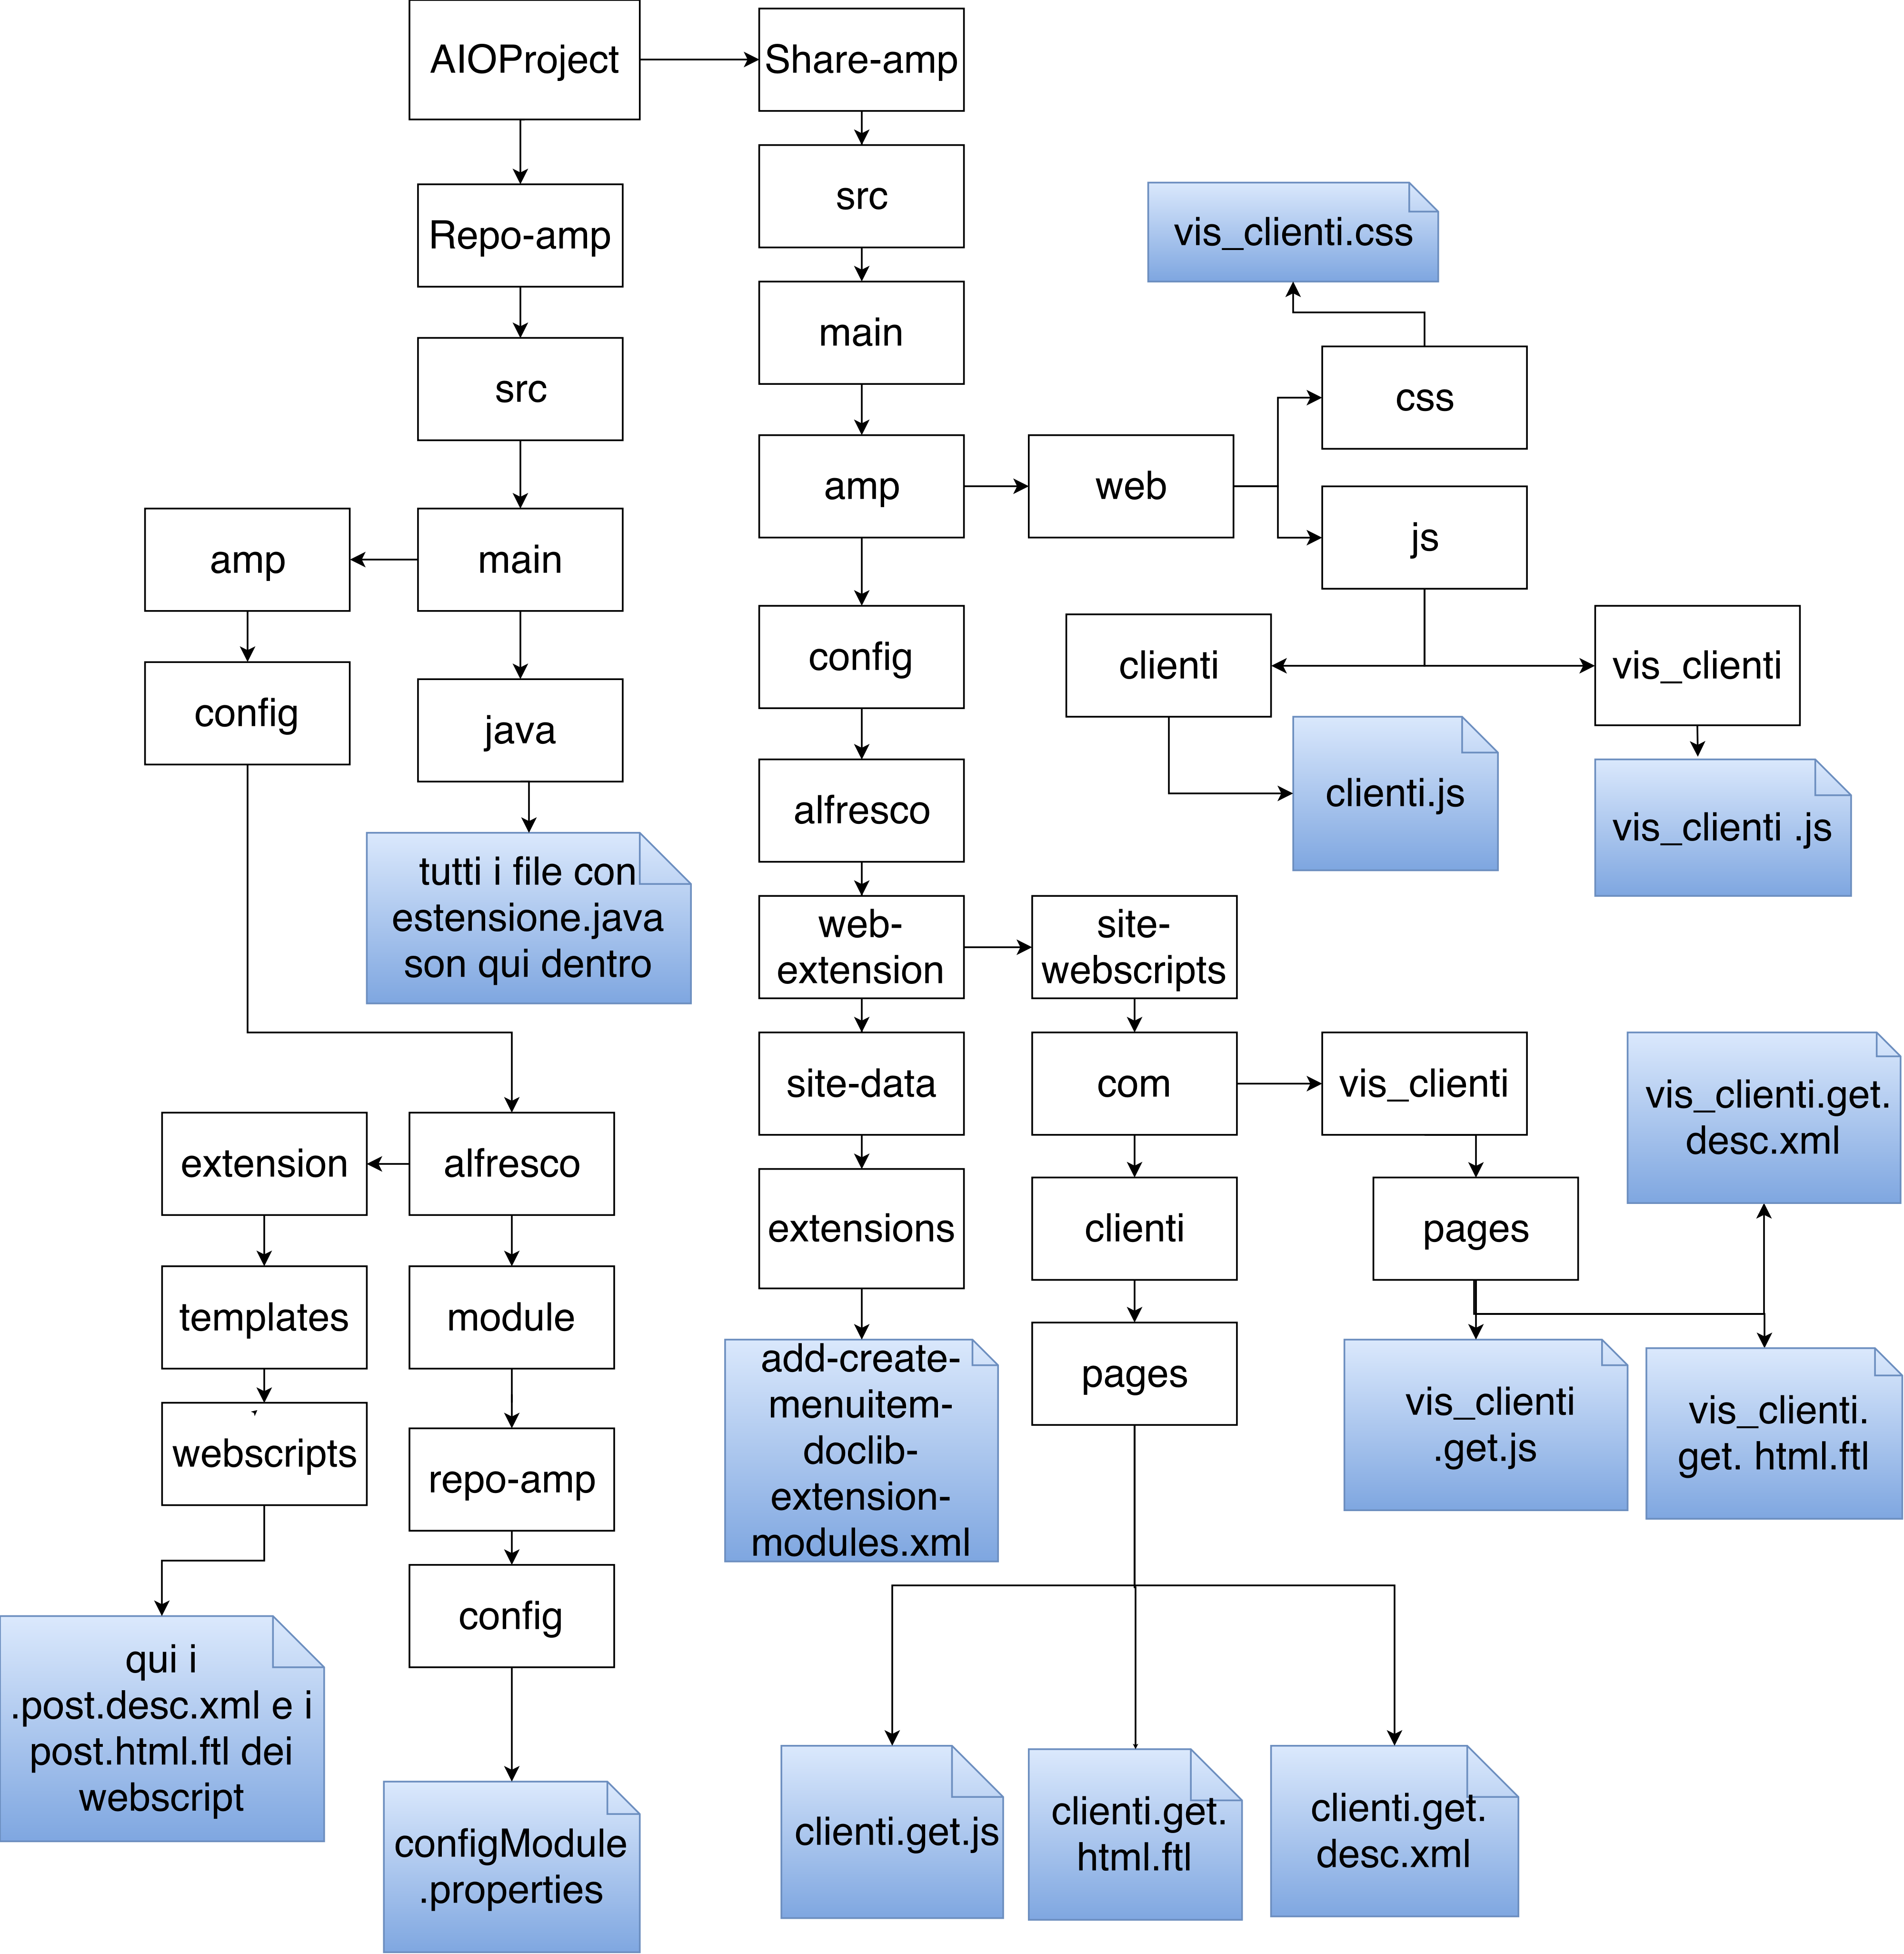
\includegraphics[width=\textwidth]{/diagrammi_cartelle/FolderClienti.png}
\caption{descrizione generale di quanto creato per il modulo relativo ai progetti\label{fig:cartelle-tema}}
\end{figure}
è stato innanzitutto aggiunto il file CoralTreeTheme.xml, il cui contenuto è riportato nel listato \ref{theme-declaration} che serve a registrare il tema
\begin{lstlisting}[language=XML, caption=XML della dichiarazione del tema, label=lst:theme-declaration]
<?xml version='1.0' encoding='UTF-8'?>
<theme>
    <title>Coral Tree Theme</title>
    <title-id>theme.CoralTreeTheme</title-id>
    <css-tokens>
        <less-variables>
            <!-- Only for Alfresco 5.x onwards and latest Aikau version -->
        </less-variables>
    </css-tokens>
</theme>
\end{lstlisting}
\subsubsection{File di funzionalità}
innanzitutto è stato creato aggiornato il file layout.js, che si occupa di gestire il tema selezionato, e il cui testo integrale è riportato nel listato \ref{code-layout}. Come si vede si controlla nelle costanti di Alfresco quale è il tema attivo e in base a quello si inietta il codice per importare i file corretti.
\begin{lstlisting}[language=JavaScript, caption=codice di layout.js, label=code-layout]
$( window ).load(function() {
    /** CoralTreeTheme **/
    if (Alfresco.constants.THEME == "CoralTreeTheme") {
        document.getElementById("HEADER_SEARCHBOX_FORM_FIELD").setAttribute("placeholder","Chi cerca, trova!");
        var arrayLink = ['/share/res/themes/CoralTreeTheme/dashboard/header/header.css', '/share/res/themes/CoralTreeTheme/dashboard/footer/footer.css'];
        for (i = 0; i < arrayLink.length; i++) {
            var link = document.createElement("link");
            link.rel = 'stylesheet';
            link.type = 'text/css';
            link.href = arrayLink[i];
            document.querySelector("head").appendChild(link);
        }
        var arrayScript = ['/share/res/js/CoralTreeTheme/dashboard/header/header.js', '/share/res/js/CoralTreeTheme/dashboard/footer/footer.js'];
        for (i = 0; i < arrayScript.length; i++) {
            var script = document.createElement("script");
            script.type= "text/javascript";
            script.src = arrayScript[i];
            document.querySelector("head").appendChild(script);
        }
        $(".yui-skin-CoralTreeTheme").css({"display":"block"});
    } else if (Alfresco.constants.THEME == "ennovaTheme") {
        var arrayLink = ['/share/res/themes/ennovaTheme/dashboard/header/header.css', '/share/res/themes/ennovaTheme/dashboard/footer/footer.css'];
        for (i = 0; i < arrayLink.length; i++) {
            var link = document.createElement("link");
            link.rel = 'stylesheet';
            link.type = 'text/css';
            link.href = arrayLink[i];
            document.querySelector("head").appendChild(link);
        }
        var arrayScript = ['/share/res/js/ennovaTheme/dashboard/header/header.js', '/share/res/js/ennovaTheme/dashboard/footer/footer.js'];
        for (i = 0; i < arrayScript.length; i++) {
            var script = document.createElement("script");
            script.type= "text/javascript";
            script.src = arrayScript[i];
            document.querySelector("head").appendChild(script);
        }
        $(".yui-skin-ennovaTheme").css({"display":"block"});
    }
});
\end{lstlisting}
\subsubsection{File di stile}
Per realizzare il tema si sono seguite le linee guida di Alfresco, che dicono di copiare i file di uno dei tema base e di lavorare su quelli, aggiungendo gli stili desiderati. Si hanno quindi:
\begin{itemize}
\item \texttt{footer.css}, che contiene il CSS specifico per il footer
\item \texttt{header.css}, che contiene il CSS specifico per l'header.
\item la cartella \texttt{images}, che contiene le immagini che sono usate dal tema
\item \texttt{presentation.css} che è il css principale del tema
\item la cartella\texttt{assets}, che contiene il css e i file necessari per i componenti yui utilizzati da Alfresco
\end{itemize}
\section{Lato estetico}
Per il lato estetico ci si è ancora una volta dovuti rivolgere al team di grafici che lavorano presso l'azienda per ottenere un mockup. Sono stati utilizzati quelli già prodotti nel passato al momento della presentazione del progetto e della creazione dei primi moduli.
\subsection{Risultati ottenuti}
TODO:immagini